%		 ** RISULTATI **

Le seguenti figure mostrano un caso potenzialmente problematico di situazione "ciclica". In tale situazione, tutti e quattro gli agenti della stanza sono occupati a tracciare un target diverso e l'inizio di un'asta potrebbe scatenare una reazione a catena senza fine. Utilizzando il protocollo d'asta implementato, la situazione si risolve con uno scambio di target.

% Figura della mappa
\begin{figure}[h]
	\centering
	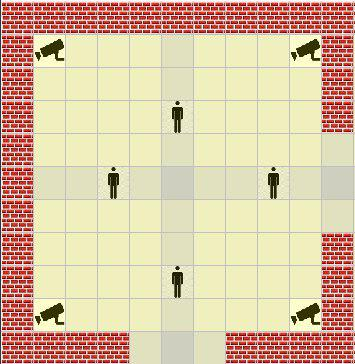
\includegraphics[width=0.3\linewidth]{room}
	\caption{Configurazione dei target ciclica.}
	\label{fig:room}
\end{figure}

% Figura della mappa
\begin{figure}[h]
	\centering
	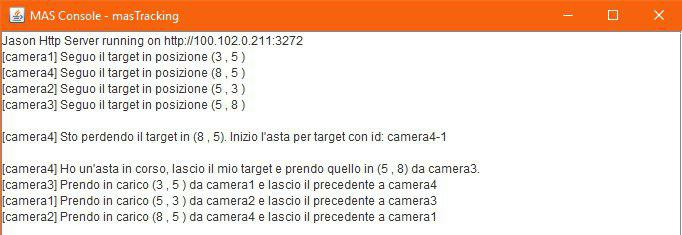
\includegraphics[width=0.7\linewidth]{console}
	\caption{Output ricevuto con la configurazione mostrata in Figura 3.}
	\label{fig:console}
\end{figure}



La tabella seguente riassume, al variare del numero di target, le seguenti statistiche:
\begin{itemize}
	\item numero medio di aste effettuate,
	\item numero medio di aste non andate a buon fine,
	\item numero medio di step in cui almeno un target non � tracciato.
\end{itemize}
\begin{center}
\begin{tabular}{| c | c | c | c |}
	\hline
	\textbf{No Target}	&	\textbf{No Aste}	&	\textbf{No Aste Fallite}	&	\textbf{No Target Persi} \\ \hline
	1	&	20	&	0	&	3	\\ \hline
	2	&	85	&	7	&	19	\\ \hline
	
\end{tabular}
\end{center}